
\chapter{Relay control systems}

The word ``discrete'' means \textit{individual} or \textit{distinct}.  In engineering, a ``discrete'' variable or measurement refers to a true-or-false condition.  Thus, a discrete control system is one designed to operate on Boolean (``on'' or ``off'') signals supplied by discrete sensors such as process switches.  \index{Discrete}

A form of discrete control taught in every introductory course on digital electronics involves the use of circuits called \textit{logic gates}.  These circuits input one or more Boolean signals, and output a Boolean signal according to a simple rule such as ``AND'' or ``OR'':  \index{Logic gate}  \index{Gate, logic}

$$\includegraphics{gate_01.eps}$$

Industrial control systems rarely utilize logic gates in a direct fashion for discrete control systems, although the fundamental \textit{concepts} of ``AND,'' ``OR,'' and other gate types are universally applied.  Instead, control functions are either implemented using electromechanical relays and/or with programmable digital devices such as PLCs (Programmable Logic Controllers).  This chapter focuses on the practical use of both technologies for industrial discrete control.  \index{PLC}  \index{Programmable Logic Controller}

\vskip 10pt

\filbreak

An ``AND'' function is equivalent to \textit{series-connected} normally-open contacts in a relay control circuit, because the lamp will energize only if switch A \textit{and} switch B are actuated:

$$\includegraphics{gate_02.eps}$$


\vskip 10pt

\filbreak

An ``OR'' function is equivalent to \textit{parallel-connected} normally-open contacts in a relay control circuit, because the lamp will energize if switch A \textit{or} switch B is actuated:

$$\includegraphics{gate_03.eps}$$


\vskip 10pt

\filbreak

The ``NOT'' function is equivalent to a single normally-closed contact in a relay control circuit, because the lamp will energize only if the switch is \textit{not} actuated:

$$\includegraphics{gate_04.eps}$$









\filbreak
\section{Control relays}

An \textit{electromechanical relay} is an electrical switch actuated by an electromagnet coil.  As switching devices, they exhibit simple ``on'' and ``off'' behavior with no intermediate states.  Relays are very useful devices, as they allow a single discrete (on/off) electrical signal to \textit{control} much greater levels of electrical power, and/or multiple power or control signals that are otherwise isolated from each other.  For example, a relay may be controlled by a low-voltage, low-current signal that passes through a delicate switch of some sort (e.g. limit switch, proximity switch, optical sensor), and then the switching contacts of that relay may be used to control a much higher-voltage, higher-current circuit, and even multiple circuits given multiple sets of switching contacts.

The electronic schematic symbol for a simple single-pole, single-throw (SPST) relay is shown here:  \index{SPST switch contacts}

$$\includegraphics{relay_01.eps}$$

A coil of wire wrapped around a laminated ferrous core provides the magnetic field necessary to actuate the switch mechanism.  This electromagnet coil's actuating influence on the relay's contact(s) is represented by the dashed line.  This particular relay is equipped with \textit{normally open} (NO) switch contacts, which means the switch will be in the open (off) state when the relay coil is de-energized.  Recall from section \ref{normal_switch} that the ``normal'' status of a switch is the resting condition of \textit{no stimulation}.  A relay switch contact will be in its ``normal'' status when its coil is not energized.  A single-pole, single-throw relay with a normally-closed (NC) switch contact would be represented in an electronic schematic like this:  \index{Normal state of a relay contact}

$$\includegraphics{relay_02.eps}$$

\filbreak

In the electrical control world, the labels ``Form-A'' and ``Form-B'' are synonymous with ``normally open'' and ``normally closed'' contacts, respectively.  Thus, we could have labeled the SPST relay contacts as ``Form-A'' and ``Form-B,'' respectively:  \index{Form-A switch contact}  \index{Form-B switch contact}

$$\includegraphics{relay_03.eps}$$

An extension of this theme is the single-pole, double-throw (SPDT) relay contact, otherwise known as a ``Form-C'' contact.  This design of switch provides both a normally-open and normally-closed contact set in one unit, actuated by the electromagnet coil:  \index{Form-C switch contact}  \index{SPDT switch contact}

$$\includegraphics{relay_04.eps}$$

A further extension on this theme is the double-pole, double-throw (DPDT) relay contact.  This design of switch provides two sets of Form-C contacts in one unit, simultaneously actuated by the electromagnet coil:  \index{DPDT switch contacts}

$$\includegraphics{relay_05.eps}$$

DPDT relays are some of the most common found in industry, due to their versatility.  Each Form-C contact set offers a choice of either normally-open or normally-closed contacts, and the two sets (two ``poles'') are electrically isolated from each other so they may be used in different circuits.

A common package for industrial relays is the so-called \textit{ice cube relay}, named for its clear plastic case allowing inspection of the working elements.  These relays plug into multi-pin base sockets for easy removal and replacement in case of failure.  A DPDT ``ice cube'' relay is shown in the following photographs, ready to be plugged into its base (left) and with the plastic cover removed to expose both sets of Form-C contacts (right):  \index{Ice cube relay}  \index{Relay, ice cube}

$$\includegraphics[width=2.5in]{relay_07.eps} \hskip 30pt \includegraphics[width=2.5in]{relay_06.eps}$$

These relays connect to the socket with eight pins: three for each of the two Form-C contact set, plus two more pins for the coil connections.  Due to the pin count (8), this style of relay base is often referred to as an \textit{octal} base.  \index{Octal base relay}

\filbreak

A closer view of one Form-C contact shows how the moving metal ``leaf'' contacts one of two stationary points, the actual point of contact being made by a silver-coated ``button'' at the end of the leaf.  The following photographs show one Form-C contact in both positions:

$$\includegraphics[width=2.5in]{relay_08.eps} \hskip 30pt \includegraphics[width=2.5in]{relay_09.eps}$$

Industrial control relays usually have connection diagrams drawn somewhere on the outer shell to indicate which pins connect to which elements inside the relay.  The style of these diagrams may vary somewhat, even between relays of identical function.  Take for instance the diagrams shown here, photographed on three different brands of DPDT relay:

$$\includegraphics[height=2.5in]{relay_10.eps} \hskip 20pt \includegraphics[height=2.5in]{relay_11.eps} \hskip 20pt \includegraphics[height=2.5in]{relay_12.eps}$$

Bear in mind that these three relays are \textit{identical} in their essential function (DPDT switching), despite differences in physical size and contact ratings (voltage and current capacities).  Only two of the three diagrams shown use the same symbols to represent contacts, and all three use unique symbols to represent the coil.

% ADD: Explain how to interpret contact diagrams -- what the NO and NC symbols mean
% ADD: 3PDT relays
% ADD: 4PDT relays











\filbreak
\section{Relay circuits}

Electromechanical relays may be connected together to perform logic and control functions, acting as logic elements much like digital gates (AND, OR, etc.).  A very common form of schematic diagram showing the interconnection of relays to perform these functions is called a \textit{ladder diagram}.  In a ``ladder'' diagram, the two poles of the power source are drawn as vertical rails of a ladder, with horizontal ``rungs'' showing the switch contacts, relay contacts, relay coils, and final control elements (lamps, solenoid coils, motors) drawn in between the power rails.

Ladder diagrams differ from regular schematic diagrams of the sort common to electronics technicians primarily in the strict orientation of the wiring: vertical power ``rails'' and horizontal control ``rungs.''  Symbols also differ a bit from common electronics notation: relay coils are drawn as circles, with relay contacts drawn in a way resembling capacitors:

$$\includegraphics[height=3in]{ladder_02.eps}$$

Unlike schematic diagrams where the association between relay coils and relay contacts is represented by dashed lines, ladder diagrams associate coils and contacts \textit{by label}.  Sometimes you will find relay contacts labeled identically to the coil (e.g. coil labeled CR5 and all contacts for that relay also labeled CR5) while other times you will find suffix numbers used to distinguish individual contacts within each relay from each other (e.g. coil labeled CR5 and its three contacts labeled CR5-1, CR5-2, and CR5-3).

Another notable convention in relay circuits and their ladder diagrams is that each and every wire in the circuit is labeled with a number corresponding to common connection points.  That is, wires connected together always bear the same number: the common number designates a condition of electrical commonality (all points bearing the same number are \textit{equipotential} to each other).  Wire numbers only change when the connection passes through a switch or other device capable of dropping voltage.

\filbreak

An actual ladder diagram of a relay-based motor control system is shown here, complete with \textit{red-line} edits showing modifications to the circuit made by an industrial electrician:  \index{Red-line editing}

$$\includegraphics[width=6in]{ladder_01.eps}$$

% ADD: elaborate on the purpose of the "PLR" relay red-lined in this drawing: to unlatch control relay R4 if ever the main power supply is shut off.

\filbreak

Perhaps the most confusing aspect of relay control circuits for students to grasp is the meaning of \textit{normal} as it applies to the status of relay contacts.  As discussed previously, the word ``normal'' in this context -- whether it be the status of hand switches, process switches, or the switch contacts inside control relays -- means ``in a condition of rest'' or no stimulation.  In other words, a ``normally-open'' relay contact is open \textit{when the relay coil is unpowered} and closed when the relay coil is powered.  Likewise, a ``normally-closed'' relay contact is closed \textit{when the relay coil is unpowered} and open when the relay coil is powered.  \index{Normal state of a relay contact}

To illustrate this concept, let us examine a relay control circuit where a pressure switch activates an alarm light:

$$\includegraphics{ladder_03.eps}$$

Here, both the pressure switch and the relay contact (CR1-1) are drawn as normally-closed switch contacts.  This means the pressure switch contact will be closed when the applied pressure is less than its trip point (50 PSI), and the relay switch contact will be closed when the relay coil is de-energized.

\vskip 10pt

\filbreak

When analyzing the operation of a relay control system, it is helpful to have some way to temporarily denote the conductive status of switch contacts and the energization status of relay coils (i.e. a notation we might sketch using pencil on a diagram to help us follow the operation of the circuit).  A symbology I recommend is the use of arrow and ``X'' symbols to represent power flow and no power flow (respectively).  These symbols clearly denote component status while avoiding confusion with the symbols used to denote \textit{normal} status of switch contacts\footnote{An unfortunately common tendency among novices is to sketch slash marks through relay contact symbols in order to show when they happen to be closed.  This is a very bad habit, and should be discouraged at all times!  Diagonal lines drawn through a contact symbol are supposed to denote the contact to be \textit{normally-}closed, not \textit{closed}: it shows that a switch contact will be in the closed (conducting) state \textit{when it is at rest}.  What we actually need is a different kind of symbol to show when a contact is closed during any arbitrary condition we may imagine.  When someone uses this same symbology to denote a contact that happens to be closed during some condition, it needlessly confuses the concepts of \textit{closed} versus \textit{normally-closed}.}.

In this next diagram, we assume the applied pressure is less than 50 PSI, leaving the pressure switch in its ``normal'' (closed) state:

$$\includegraphics{ladder_04.eps}$$

Since the pressure is insufficient to actuate the pressure switch, its contact remains in the ``normal'' state (closed).  This sends power to relay coil CR1, thus actuating contact CR1-1 and holding it in the \textit{open} state.  With CR1-1 contact open, the alarm lamp receives no power.  In this example we see the pressure switch in its ``normal'' state but the relay in the \textit{actuated} state.

\vskip 10pt

\filbreak

Using arrow and ``X'' symbols again to represent the presence or absence of power in this circuit, we will now analyze its status with an applied switch pressure greater than 50 PSI:

$$\includegraphics{ladder_05.eps}$$

Now that there is sufficient fluid pressure applied to the switch to actuate it, its contact is forced into the actuated state which for this ``normally-closed'' switch is open.  This open condition de-energizes relay coil CR1, allowing relay contact CR1-1 to spring-return to its normal status (closed), thus sending power to the alarm lamp.  From this analysis we see that the lamp fulfills the function of a \textit{high pressure alarm}, energizing when the applied pressure exceeds the trip point.

\vskip 10pt

Where students typically find themselves confused is assuming the switch contact will be in the same state it is drawn in.  This is not necessarily true.  The way switch contacts are drawn merely reflects their \textit{normal} status as defined by the switch manufacturer, which means the status of the switch when there is no (or insufficient) actuating stimulus present.  Whether or not the switch will actually be in its normal state at any given time is a question of whether or not a sufficient stimulus is present to actuate that switch.  Just because a switch is drawn normally-closed does not necessarily mean it \textit{will} be closed when you go to analyze it.  All it means is that the switch will be closed \textit{when nothing actuates it}.

\vskip 10pt

This exact same principle applies to relay ladder-logic programming in electronic control systems called PLCs (Programmable Logic Controllers).  In a PLC, a digital microprocessor performs the logic functions traditionally provided by electromechanical relays, with the programming for this microprocessor taking the form of a relay diagram (also called a ``ladder-logic'' diagram).   \index{Ladder Diagram programming}  \index{LD}  \index{Relay Ladder Logic programming}  \index{RLL} 

\filbreak

Here, we will emulate the exact same high-pressure alarm circuit using an Allen-Bradley MicroLogix 1000 PLC instead of a relay coil:  \index{Programmable Logic Controller}  \index{PLC}

\vskip 10pt

\noindent
\textbf{Wiring diagram:}

$$\includegraphics{ladder_06.eps}$$

\noindent
\textbf{Ladder-logic program:}

$$\includegraphics[width=6in]{ladder_07.eps}$$

Suppose a fluid pressure of 36 PSI is applied to the pressure switch.  This is less than the switch's trip setting of 50 PSI, leaving the switch in its ``normal'' (closed) state.  This sends power to input \texttt{I:0/2} of the PLC.  The contact labeled \texttt{I:0/2} drawn in the ladder-logic program of the PLC acts like a relay contact driven by a coil energized by input terminal \texttt{I:0/2}.  Thus, the closed pressure switch contact energizes input terminal \texttt{I:0/2}, which in turn ``closes'' the normally-open contact symbol \texttt{I:0/2} drawn in the ladder-logic program.  This ``virtual'' contact sends virtual power to a virtual coil labeled \texttt{B3:0/0}, which is nothing more than a single bit of data in the PLC's microprocessor memory.  ``Energizing'' this virtual coil has the effect of ``actuating'' any contact drawn in the program bearing the same label.  This means the normally-closed contact \texttt{B3:0/0} will now be ``actuated'' and thus in the open state, not sending virtual power to the output coil \texttt{O:0/1}.  With virtual coil \texttt{O:0/1} ``unpowered,'' the real-life output \texttt{O:0/1} on the PLC will be electrically open, and the alarm lamp will be unpowered (off).  \index{Normal state of a PLC program contact}

If we apply a fluid pressure of 61 PSI to the pressure switch, the normally-closed pressure switch contact will be actuated (forced) into the open state.  This will have the effect of de-energizing PLC input \texttt{I:0/2}, thus ``opening'' the normally-open virtual contact in the PLC program bearing the same label.  This ``open'' virtual contact interrupts virtual power to the virtual coil \texttt{B3:0/0}, causing the normally-closed virtual contact \texttt{B3:0/0} to ``close,'' sending virtual power to virtual coil \texttt{O:0/1}.  When this virtual output coil ``energizes,'' the real-life output channel of the PLC activates, sending real power to the alarm light to turn it on, signaling a high-pressure alarm condition.

We may simplify this PLC program further by eliminating the virtual control relay \texttt{B3:0/0} and simply having input \texttt{I:0/2} activate output \texttt{O:0/1} through a ``normally-closed'' virtual contact:

$$\includegraphics[width=6in]{ladder_08.eps}$$

The effect is the same: the PLC output \texttt{O:0/1} will activate whenever input \texttt{I:0/2} de-energizes (whenever the pressure switch is opened by a high pressure), turning on the alarm lamp in a high-pressure condition.  In a low-pressure condition, the energized input \texttt{I:0/2} forces the virtual normally-closed contact \texttt{I:0/2} to open, thus de-energizing the PLC's output \texttt{O:0/1} and turning the alarm lamp off.

\vskip 10pt

Programmable Logic Controllers have not only greatly simplified the wiring of industrial logic controls by replacing multitudes of electromechanical relays with a microprocessor, but they have also added advanced capabilities such as counters, timers, sequencers, mathematical functions, communications, and of course the ability to easily modify the control logic through programming rather than by re-wiring relays.  The beauty of ladder-logic programming is that it translates the technician's understanding of traditional relay control circuits into a virtual form where contacts and coils interact to perform practical control functions.  A key concept to master, however, is the association of real-life conditions to switch status based on the ``normal'' representation of those switch contacts, whether the switches be real (relay) or virtual (PLC).  Once this vital concept is mastered, both hard-wired relay control circuits and PLC programs become possible to understand.  Without mastering this vital concept, neither relay control circuits nor PLC programs may be understood.












\filbreak
\section{Interposing relays}

In addition to directly performing logic functions, electromechanical relays may also be used as \textit{interposing} devices between mismatched sensors, controllers, and/or control devices.  A very simple example of a relay used to interpose between mismatched devices is shown in the following circuit diagram, where a delicate toggle switch is used to control a bank of high-power lights for an off-road vehicle:

$$\includegraphics{relay_14.eps}$$

In this circuit the relay performs no logic function whatsoever.  Rather, it merely ``amplifies'' the signal sent by the dashboard toggle switch to send or halt power to the bank of high-power lights.  Without the relay, a much heavier-duty toggle switch would have to be installed in the dashboard of this vehicle to safely and reliably make and break the light circuit.

Another example of an interposing relay found in automotive applications is the use of a ``solenoid'' in the electric starting motor circuit for an internal combustion engine.  The ``start'' control switch is typically actuated by the driver turning a key, that switch mounted on the steering column or dashboard of the vehicle.  The starting motor, meanwhile, typically draws \textit{hundreds of amps} of current as it labors to start up the engine.  A keyswitch capable of making and breaking hundreds of amps of current would be enormous, and in fact dangerous to locate in the cab of the vehicle.  The ``solenoid'' relay connected between the keyswitch and the starting motor relocates that danger, and allows a relatively delicate keyswitch to safely activate the high-power motor.

\vskip 10pt

\filbreak

An industrial example of an interposing relay between mismatched devices is shown here, where a DC output proximity switch must trigger an input channel to a Programmable Logic Controller (PLC) rated for 120 volts AC:  \index{Interposing}  \index{Programmable Logic Controller}  \index{PLC}

$$\includegraphics{relay_13.eps}$$

Again, the relay in this system performs no logic function, but merely allows the proximity switch to drive one of the PLC input channels.  Directly connecting the proximity switch to one of the input channels of the PLC is not a practical option, because this particular PLC input requires 120 volts AC to activate, and our proximity switch operates on 24 volts DC.  The mismatch between switch voltage and PLC input voltage requires us to use the relay to ``interpose'' between the switch and PLC.  When the proximity switch senses an object nearby, its output activates, which in turn energizes the relay coil.  When the relay contact magnetically closes, it completes a circuit for 120 volts AC to reach input channel 0 on the PLC, thereby energizing it.

\vskip 10pt

An important detail in this relay circuit is the inclusion of a \textit{commutating diode} in parallel with the relay coil, the purpose being to dissipate the coil's stored energy upon de-energization when the proximity switch turns off.  Without this diode in place, the coil's ``kickback'' voltage (which may reach hundreds of volts in potential) will destroy the proximity switch's output transistor.  \index{Commutating diode}  \index{Diode, commutating}

Note how this commutating diode appears to be connected ``backwards'' with regard to the polarity of the 24 volt DC power source: cathode toward the source's positive pole and anode toward the source's negative pole.  This is intentional, as we do \textit{not} wish to have the diode conduct when power is applied to the relay coil through the proximity switch\footnote{If the diode were connected the other way, it would pass current whenever the proximity switch turned on, shorting past the relay coil and most likely damaging the proximity switch in doing so!}.  The diode only turns on when the polarity reverses, which is what happens when the proximity switch turns off and the relay coil's magnetic field collapses (now acting as a source rather than as a load).  As the relay coil temporarily outputs a ``reverse'' voltage, the diode gives that coil a continuous path for its current while dropping a low voltage (about 0.7 volts DC), dissipating the coil's stored energy in the form of heat at the diode.

\vskip 10pt

\filbreak

Interposing relays are also used to connected mismatched PLC outputs and control devices.  In this application, the mismatch may be in terms of voltage ratings and/or current ratings.  As with the input interposing circuit shown previously, the task of the relay in an output interposing circuit is to be controlled by the PLC's output channel, and in turn direct power to a field device that is itself incompatible with the PLC's output.

The following diagram shows an example of an interposing relay connected to a PLC output channel:

$$\includegraphics{relay_15.eps}$$

In this circuit the PLC's transistor outputs can only handle 24 volts DC, and at fairly low current.  The three-phase contactor\footnote{A ``contactor'' is nothing more than a very large electromechanical relay, and itself is a form of interposing device.  Its purpose is to make and break three-phase AC power to a heavy load (e.g. an electric motor) at the command of a much smaller electrical signal, in this case a 120 volt AC signal sent to the coil of the contactor.} coil requires 120 volts AC at modest current levels to function, and so the relay interposes between the PLC's low-voltage and low-current output channel and the relatively high-voltage and high-current demands of the contactor's coil.  Once again we see the use of a commutating diode to dissipate the relay coil's stored energy whenever the PLC de-energizes it, so that the resulting ``kickback'' voltage does not damage the fragile transistor output circuitry within the PLC.  \index{Contactor}








\filbreak
\section{Review of fundamental principles}

Shown here is a partial listing of principles applied in the subject matter of this chapter, given for the purpose of expanding the reader's view of this chapter's concepts and of their general inter-relationships with concepts elsewhere in the book.  Your abilities as a problem-solver and as a life-long learner will be greatly enhanced by mastering the applications of these principles to a wide variety of topics, the more varied the better.

\begin{itemize}
\item \textbf{Amplification}: the control of a relatively large signal by a relatively small signal.  Relevant to the role of relays as interposing devices.
\item \textbf{Interposing}: the use of a relay as an intermediary between electrically incompatible devices.
\item \textbf{``Normal'' switch status}: the ``normal'' status of a switch contact as defined by the manufacturer is its \textit{resting} condition (minimum stimulus).
\item \textbf{``Seal-in'' circuit}: when an electrical relay uses one of its own switch contacts to continue its own coil energization after the initial triggering event has passed.  Relevant to all manner of relay control circuits.
\end{itemize}













\filbreak
\section*{References}

% In alphabetical order!
% \noindent
% Lastname, Firstname MiddleI., \textit{Book Title}, Publisher, City, State, Year.
% \vskip 10pt
% \noindent
% Lastname, Firstname MiddleI., \textit{Book Title}, Publisher, City, State, Year.
% etc . . .

\noindent
Summers, Wilford I. and Croft, Terrell, \textit{American Electrician's Handbook}, Eleventh Edition, McGraw-Hill Book Company, New York, NY, 1987.


















%%%%%%%%%%%%%%%%%%%%%%%%%%%%%%%%%%%%%%%%%%%%%%%%%%%%

